  \centering
  \begin{minipage}[c]{0.4\textwidth}
    \centering
    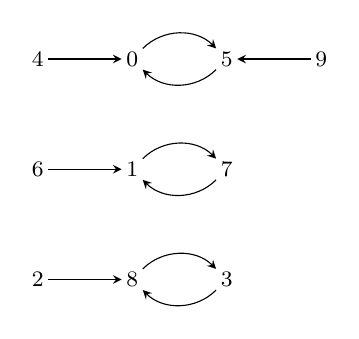
\begin{tikzpicture}[>=stealth, font=\footnotesize,
        every node/.style={inner sep=1.5pt}]
      % Component 1: 4 -> 0 <=> 5 <- 9
      \node (n4) at (0,0)     {$4$};
      \node (n0) at (1.2,0)   {$0$};
      \node (n5) at (2.4,0)   {$5$};
      \node (n9) at (3.6,0)   {$9$};
      % Component 2: 6 -> 1 <=> 7
      \node (n6) at (0,-1.4)   {$6$};
      \node (n1) at (1.2,-1.4) {$1$};
      \node (n7) at (2.4,-1.4) {$7$};
      % Component 3: 2 -> 8 <=> 3
      \node (n2) at (0,-2.8)   {$2$};
      \node (n8) at (1.2,-2.8) {$8$};
      \node (n3) at (2.4,-2.8) {$3$};

      \draw[->] (n4) -- (n0);
      \draw[->] (n9) -- (n5);
      \draw[->] (n0) to[bend left=45] (n5);
      \draw[->] (n5) to[bend left=45] (n0);

      \draw[->] (n6) -- (n1);
      \draw[->] (n1) to[bend left=45] (n7);
      \draw[->] (n7) to[bend left=45] (n1);

      \draw[->] (n2) -- (n8);
      \draw[->] (n8) to[bend left=45] (n3);
      \draw[->] (n3) to[bend left=45] (n8);
    \end{tikzpicture}
  \end{minipage}%
  \hfill
  \begin{minipage}[c]{0.58\textwidth}
  \centering
  {
  \newcommand{\nodea}{\node[draw=none, inner sep=2pt] (a) {}
  ;}
  \newcommand{\nodeb}{\node[draw=none, inner sep=2pt] (b) {}
  ;}
  \newcommand{\nodec}{\node[draw=none, inner sep=2pt] (c) {}
  ;}
  \newcommand{\noded}{\node[draw=none, inner sep=2pt] (d) {}
  ;}
  \newcommand{\nodee}{\node[draw=none, inner sep=2pt] (e) {}
  ;}
  \newcommand{\nodef}{\node (f) {$\overline{11}$}
  ;}
  \newcommand{\nodeg}{\node (g) {$\overline{10}$}
  ;}
  \newcommand{\nodeh}{\node (h) {$\overline{9}$}
  ;}
  \newcommand{\nodei}{\node (i) {$\overline{8}$}
  ;}
  \newcommand{\nodej}{\node (j) {$\overline{7}$}
  ;}
  \newcommand{\nodek}{\node (k) {$\overline{6}$}
  ;}
  \newcommand{\nodel}{\node (l) {$\overline{5}$}
  ;}
  \newcommand{\nodem}{\node (m) {$\overline{4}$}
  ;}
  \newcommand{\noden}{\node (n) {$\overline{3}$}
  ;}
  \newcommand{\nodeo}{\node (o) {$\overline{2}$}
  ;}
  \newcommand{\nodep}{\node (p) {$\overline{1}$}
  ;}
  \newcommand{\nodeq}{\node (q) {$0$}
  ;}
  \newcommand{\noder}{\node (r) {$1$}
  ;}
  \newcommand{\nodes}{\node (s) {$2$}
  ;}
  \newcommand{\nodet}{\node (t) {$3$}
  ;}
  \newcommand{\nodeu}{\node (u) {$4$}
  ;}
  \newcommand{\nodev}{\node (v) {$5$}
  ;}
  \newcommand{\nodew}{\node (w) {$6$}
  ;}
  \newcommand{\nodex}{\node (x) {$7$}
  ;}
  \newcommand{\nodey}{\node (y) {$8$}
  ;}
  \newcommand{\nodez}{\node (z) {$9$}
  ;}
  \newcommand{\nodeaa}{\node (aa) {$10$}
  ;}
  \newcommand{\nodeab}{\node (ab) {$11$}
  ;}
  \newcommand{\nodeac}{\node (ac) {$12$}
  ;}
  \newcommand{\nodead}{\node (ad) {$13$}
  ;}
  \newcommand{\nodeae}{\node[draw=none, inner sep=2pt] (ae) {}
  ;}
  \newcommand{\nodeaf}{\node[draw=none, inner sep=2pt] (af) {}
  ;}
  \newcommand{\nodeag}{\node[draw=none, inner sep=2pt] (ag) {}
  ;}
  \newcommand{\nodeah}{\node[draw=none, inner sep=2pt] (ah) {}
  ;}
  \newcommand{\nodeai}{\node[draw=none, inner sep=2pt] (ai) {}
  ;}
  \begin{tikzpicture}[auto, font=\footnotesize]
  \matrix[column sep=.3cm, row sep=.5cm,ampersand replacement=\&]{
    \nodea  \&  \nodeb  \&  \nodec  \&  \noded  \&           \&  \nodee  \\
    \nodef  \&  \nodeg  \&           \&  \nodeh  \&  \nodei  \&  \nodej  \\
    \nodek  \&  \nodel  \&  \nodem  \&  \noden  \&           \&  \nodeo  \\
    \nodep  \&  \nodeq  \&           \&  \noder  \&  \nodes  \&  \nodet  \\
    \nodeu  \&  \nodev  \&  \nodew  \&  \nodex  \&           \&  \nodey  \\
    \nodez  \&  \nodeaa  \&           \&  \nodeab  \&  \nodeac  \&  \nodead  \\
    \nodeae  \&  \nodeaf  \&  \nodeag  \&  \nodeah  \&           \&  \nodeai  \\
  };

  \path[ultra thick]   (g) edge (k)
  	  (g) edge (l)
  	  (h) edge (m)
  	  (h) edge (n)
  	  (j) edge (o)
  	  (l) edge (p)
  	  (l) edge (q)
  	  (n) edge (r)
  	  (o) edge (s)
  	  (o) edge (t)
  	  (q) edge (u)
  	  (q) edge (v)
  	  (r) edge (w)
  	  (r) edge (x)
  	  (t) edge (y)
  	  (v) edge (z)
  	  (v) edge (aa)
  	  (x) edge (ab)
  	  (y) edge (ac)
  	  (y) edge (ad);
  \path[ultra thick, dotted]   (b) edge (f)
  	  (b) edge (g)
  	  (d) edge (h)
  	  (e) edge (i)
  	  (e) edge (j)
  	  (aa) edge (ae)
  	  (aa) edge (af)
  	  (ab) edge (ag)
  	  (ab) edge (ah)
  	  (ad) edge (ai);
  \end{tikzpicture}}
  \end{minipage}
